
%***************************************************************************
%
% CreditCruncher - A portfolio credit risk valorator
% Copyright (C) 2005 Gerard Torrent
%
% This program is free software; you can redistribute it and/or
% modify it under the terms of the GNU General Public License
% as published by the Free Software Foundation; either version 2
% of the License.
%
% This program is distributed in the hope that it will be useful,
% but WITHOUT ANY WARRANTY; without even the implied warranty of
% MERCHANTABILITY or FITNESS FOR A PARTICULAR PURPOSE.  See the
% GNU General Public License for more details.
%
% You should have received a copy of the GNU General Public License
% along with this program; if not, write to the Free Software
% Foundation, Inc., 59 Temple Place - Suite 330, Boston, MA 02111-1307, USA.
%
%
% introduction.tex - TeX documentation file
% --------------------------------------------------------------------------
%
% 2005/04/17 - Gerard Torrent [gerard@fobos.generacio.com]
%   . initial release
%
%***************************************************************************

\chapter{Ejemplos}
\label{sec:examples}

Los ejemplos de este cap\'itulo se encuentran incluidos en el directorio
\verb+samples+ de la distribuci\'on de CreditCruncher y son reproducibles.

\section{C\'opula Normal}

\begin{figure}[!hb]
\begin{center}

\includegraphics[height=5cm, angle=0]{./images/copula.eps}
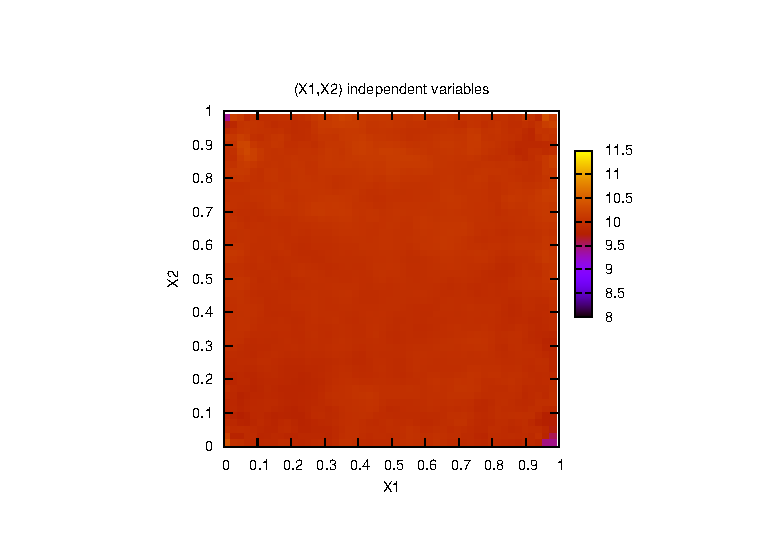
\includegraphics[height=5cm, angle=0]{./images/uniform.eps}
\caption{Bivariate distribution plot with correlated and uncorrelated variables}
\label{copulas}
\end{center}
\end{figure}


\section{Impacto de la correlaci\'on intrasectorial}

Deseamos comprobar el impacto de la correlaci\'on entre los clientes de la 
cartera. Para ello dise\~namos el siguiente escenario:

\begin{itemize}
\item M\'etodo de resoluci\'on: Rating Path
\item N\'umero de clientes: 100
\item N\'umero de sectores: 1
\item Fecha inicial: 01/01/2005
\item N\'umero de pasos temporales: 1
\item Longitud del paso: 12 meses
\item N\'umero de simulaciones: 5000
\item N\'umero de activos: 100 (uno por cliente)
\item Caracter\'isticas de los activos: valen 1 si el cliente est\'a vivo, 0 si 
ha hecho fallido
\end{itemize}

Realizamos una simulaci\'on considerando que los fallidos son independientes y 
realizamos otra simulaci\'on considerando que existe una correlaci\'on de
$0.2$. En la figura \ref{sectorcorrel} se muestra las distribuciones del 
valor de las carteras obtenidos.

\begin{figure}[!hb]
\begin{center}
\includegraphics[width=6cm,angle=-90]{./samples/sectorcorrel.ps}
\caption{Impacto de la correlaci\'on intrasectorial}
\label{sectorcorrel}
\end{center}
\end{figure}

Los ficheros de entrada correspondientes son \verb+samples/sample01.xml+ y 
\verb+samples/sample02.xml+.

\section{Impacto de la correlaci\'on intersectorial}

